\documentclass[a4paper, 12pt, english]{article}
\usepackage[utf8]{inputenc}
\usepackage{fancyhdr}
\usepackage{graphicx}
\usepackage{lastpage}
\usepackage{layout}
\usepackage{enumitem}
\usepackage{etoolbox}
\usepackage{mathptmx}
\usepackage[bottom]{footmisc}
\usepackage[includeheadfoot, left=3cm, right=3cm, top = 1.5 cm]{geometry}

\graphicspath{ {./answers/} }

\pagestyle{fancy}
\fancyhf{} 
\rhead{
    {\Large \textbf{Analysis and Design of Algorithms}}\\
    \textbf{CS2102} \\ 
    \textbf{Asymptotic Analysis Practice} \\ 
    \textbf{2020-II}
}
\lhead{
\includegraphics[width=4.6cm, keepaspectratio]{logo/utec}}
\rfoot{\textbf{\thepage}\hspace{1pt} of \textbf{\pageref{LastPage}}}
\cfoot{}

\setlength{\parindent}{0em}
\setlength{\headheight}{80pt}

\newcounter{problem}[section]
\newenvironment{problem}[3][]{\refstepcounter{problem}\par\medskip 

\textbf{Problem~\theproblem  ~~(#2) - 
\ifboolexpr{
  test {\ifdimless{1 pt}{#3 pt}}
}
{#3 points} % true
{#3 point} % false
} \newline\newline } {\medskip} 


\begin{document}

\textbf{Duration}: 100 minutes\\ 
\textbf{Number of questions}: 5

\begin{itemize}
    \item Attach your answers in order to keep a single PDF file. Your images should be located inside the \emph{answers} folder and every image should have the name:  \emph{problem\{1,2,3,4,5\}.\{pdf,png,jpg\}} based on the problem you are solving. At the end there is an example of how to attach your answers in \LaTeX.
    \item Read the questions carefully and write your answers clearly. Answers that are not legible will not have any score. 
    \item Notes are allowed. To compile this file you can use the command latexmk -pdf main.tex
\end{itemize}

\underline{Outcomes}:

\begin{enumerate}[label=\alph*.]
    \item Apply appropriate mathematical and related knowledge to computer science.
    \item Analyze problems and identify the appropriate computational requirements for its solution.
\end{enumerate}
\noindent\rule{\textwidth}{0.01pt}

\vspace{5mm}

\begin{problem}{Outcomes b}{2}
    The insertion sort implementation provided in the lectures uses linear search to find the position where an element should be inserted into the already sorted part of the array ($<k$). Consider that we replace the linear search with a binary search algorithm, what will be the new complexity for the worst case running time? Explain your answer
\end{problem}

\begin{problem}{Outcomes a, b}{8}
    Tower of Hanoi is a mathematical puzzle that consists of 3 rods where one of them is composed by a stack of n disks arranged from largest on the bottom to smallest on top. The objective of the puzzle is to move the entire stack of disks from one rod to another given the following constraints: i) you can only move one disk at a time and ii) a larger disk can never lie above a smaller disk.

    \begin{enumerate}[label=(\roman*)]
        \item Write a recursive algorithm to solve the Tower of Hanoi puzzle.
        \item Analyze and explain the proof of correctness of your algorithm.
        \item Sketch the recursion tree and calculate $T(n)$ based on the costs of each level.
        \item Write the recurrence equation and solve it using induction or master method, if possible.
    \end{enumerate}
\end{problem}

\begin{problem}{Outcome a}{4}
    Prove or disprove the following expresions:
    \begin{enumerate}[label=(\roman*)]
        \item $T(n) = \Theta(T(n))$
        \item $T(n) = \Theta(g(n))$ and $g(n) = \Theta(h(n))$ implies $T(n) = \Theta(h(n))$
        \item $T(n) = \Theta(f(n))$ implies $f(n) = \Theta(T(n))$
        \item For any 2 numbers $a,b$ one of the following \textbf{must} hold: $a<b$, $a=b$, $a>b$. Given 2 functions $T(n), f(n)$ is it true that always one of the following holds? $T(n)=\Theta(f(n))$, $T(n)=o(f(n))$, $T(n)=\omega(f(n))$
    \end{enumerate}
\end{problem}

\begin{problem}{Outcome a}{4}
    Use substitution method to solve the following expressions:
    \begin{enumerate}[label=(\roman*)]
        \item $T(n) = T(\lceil n/2 \rceil) + T(\lfloor n/2 \rfloor) + \Theta(n)$
        \item $T(n) = T(n/5) + T(3n/4) + \Theta(n)$
    \end{enumerate}
\end{problem}

\begin{problem}{Outcome a}{2}
    Consider $T(n) = 4T(n/2) + f(n)$ where $f(n) = n^{2}log(n)$, show if $f(n)$ is polynomically greater than $n^{log_b a}$. If that is true solve the expression using master theorem, otherwise propose an upper and lower bound to $T(n)$
\end{problem}

\begin{figure}[h]
    \centering
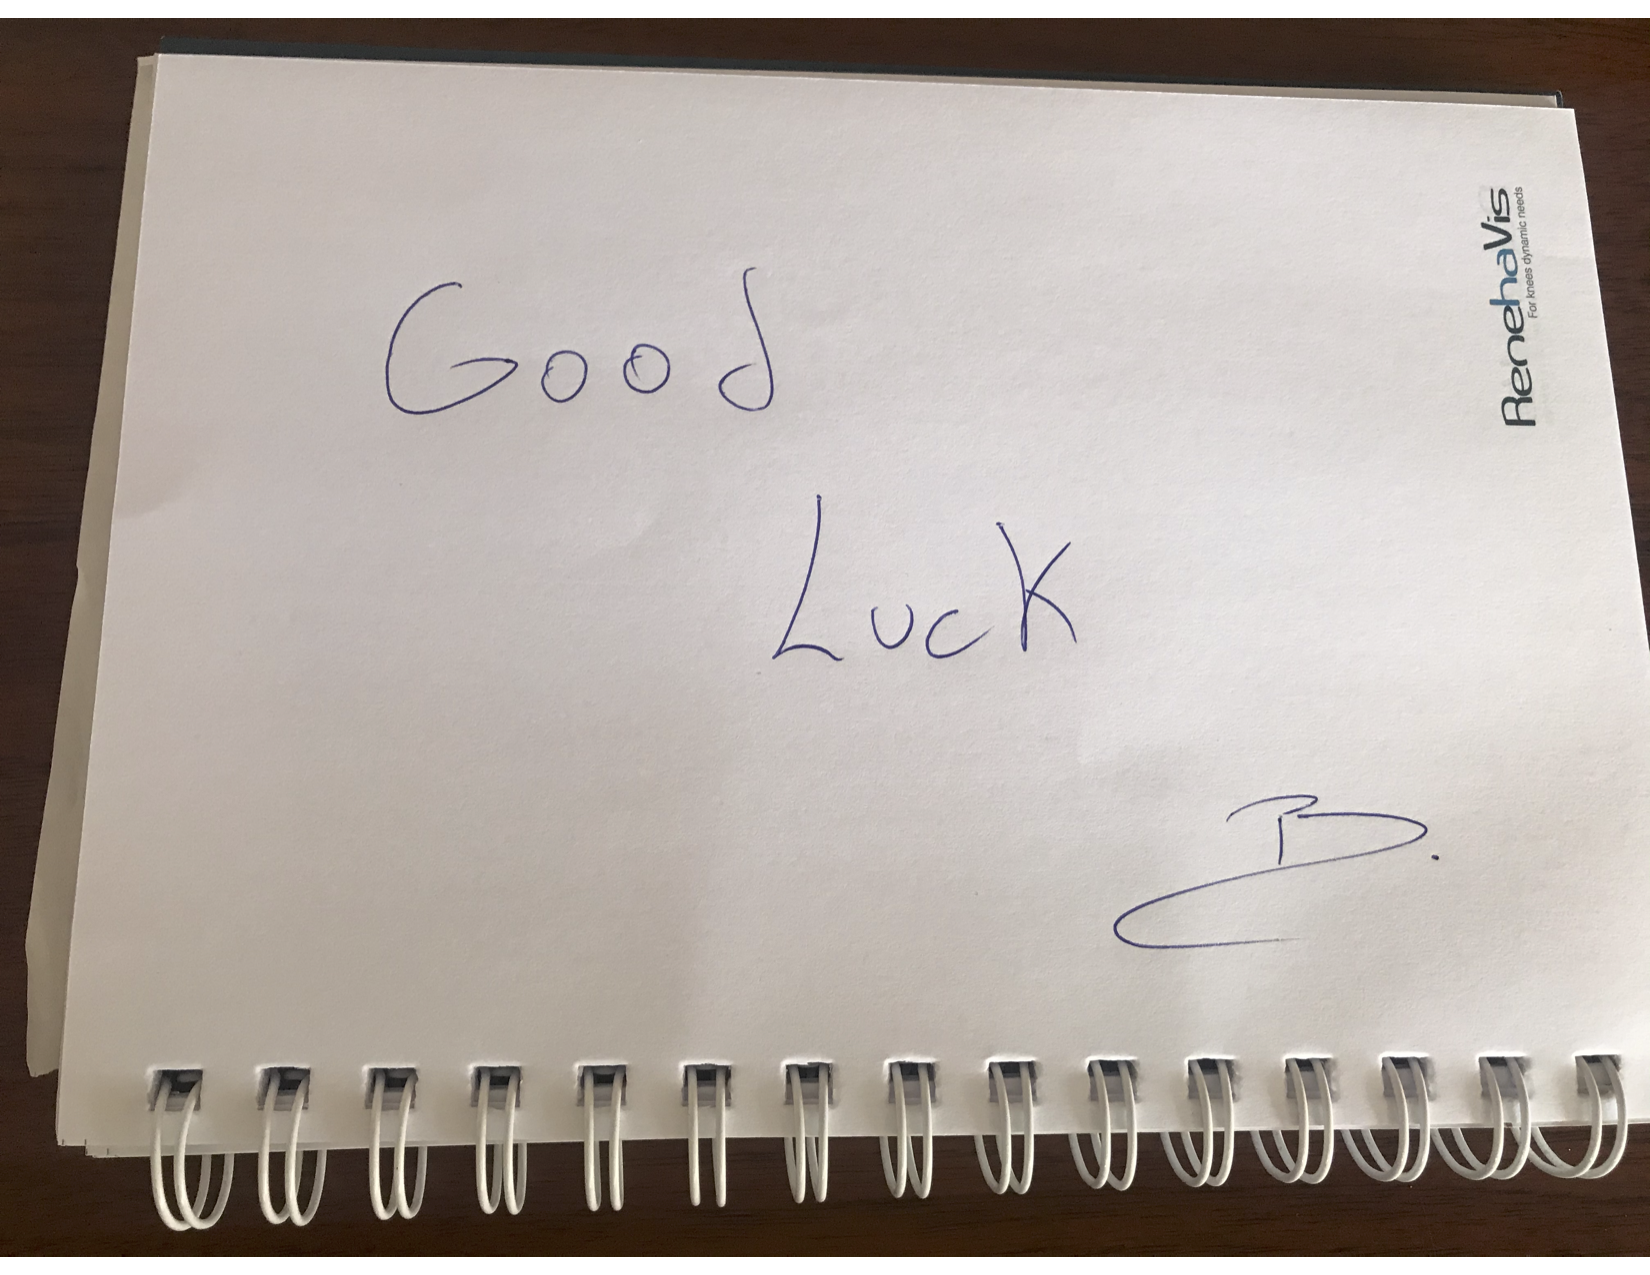
\includegraphics[width=0.7\textwidth]{sample}
\end{figure}

\end{document}
